\newcommand{\EMThreeFigOne}{%
\begin{center}
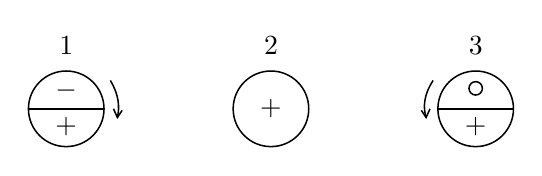
\begin{tikzpicture}[x=1cm,y=1cm,line width=.55pt]
\draw (0,0) circle (.48);\draw (-.48,0)--(.48,0);
\node at (0,.80){1};\node at (0,.23){$-$};\node at (0,-.23){$+$};
\draw (.56,.36) .. controls (.67,.18) and (.68,.02) .. (.65,-.11);
\draw (.60,.00)--(.65,-.11)--(.71,-.02);
\draw (2.6,0) circle (.48);\node at (2.6,.80){2};\node at (2.6,0){$+$};
\draw (5.2,0) circle (.48);\draw (4.72,0)--(5.68,0);
\node at (5.2,.80){3};\draw (5.2,.26) circle (.085);\node at (5.2,-.23){$+$};
\draw (4.66,.36) .. controls (4.54,.18) and (4.53,.02) .. (4.57,-.11);
\draw (4.51,-.02)--(4.57,-.11)--(4.62,.00);
\end{tikzpicture}\par\smallskip\textbf{Figur 1.}
\end{center}}
\newcommand{\EMThreeFigTwo}{%
\begin{center}
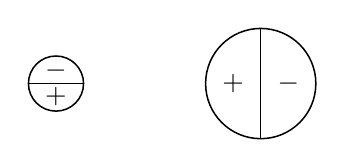
\begin{tikzpicture}[x=1cm,y=1cm,line width=.55pt]
\draw (0,0) circle (.35);\draw (-.35,0)--(.35,0);
\node at (0,.17){$-$};\node at (0,-.17){$+$};
\draw (2.6,0) circle (.7);\draw (2.6,-.7)--(2.6,.7);
\node at (2.25,0){$+$};\node at (2.95,0){$-$};
\end{tikzpicture}\par\smallskip\textbf{Figur 2.}
\end{center}}
\newcommand{\EMThreeFigThree}{%
\begin{center}
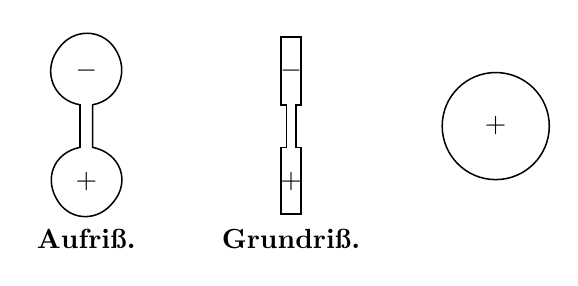
\begin{tikzpicture}[x=1cm,y=1cm,line width=.55pt]
\draw (-.08,.28)--(-.08,.82)
 .. controls (-.43,.88) and (-.57,1.27) .. (-.34,1.55)
 .. controls (-.16,1.79) and (.19,1.79) .. (.36,1.54)
 .. controls (.56,1.25) and (.41,.88) .. (.08,.82)
 --(.08,.28)
 .. controls (.43,.21) and (.57,-.15) .. (.34,-.42)
 .. controls (.15,-.66) and (-.18,-.66) .. (-.35,-.42)
 .. controls (-.55,-.13) and (-.42,.21) .. cycle;
\node at (0,1.25){$-$};\node at (0,-.16){$+$};
\node[below] at (0,-.64){\textbf{Aufriß.}};
\draw (2.47,1.68)--(2.73,1.68)--(2.73,.82)--(2.66,.82)--(2.66,.28)--(2.73,.28)--(2.73,-.57)--(2.47,-.57)--(2.47,.28)--(2.54,.28)--(2.54,.82)--(2.47,.82)--cycle;
\node at (2.6,1.25){$-$};\node at (2.6,-.16){$+$};
\node[below] at (2.6,-.64){\textbf{Grundriß.}};
\draw (5.2,.55) circle (.68);\node at (5.2,.55){$+$};
\end{tikzpicture}\par\smallskip\textbf{Figur 3.}
\end{center}}
